\section{Estimacion de variables peatonales}

Nuestro objetivo es estimar y calcular ciertas métricas por período de tiempo
(el cálculo es posible hacerlo por hora, por día, por semana).
Hemos priorizado en las definiciones de las variables peatonales 
y métodos de cálculo que se garantice la coherencia interna, en otras palabras
dado un período de tiempo que empieza y termina con el local vacío.

%\subsection{Definiciones}

Sean $V_T$ las visitas totales, $\overline{Oc}$ y $\overline{Tp}$ 
la ocupación y el tiempo de permanencia promedios durante el período $T$

\begin{equation} 
   \frac{\overline{Oc}}{\overline{Tp}} = \frac{V_T}{T}
   \label{eq:OcTpVT}
\end{equation}

\subsection{Circulación exterior en el pasillo}
La circulación exterior $C$ la detectamos con un sensor Clarity ubicado en el pasillo,
considerando el Área del local $L$ y el Área de detección donde está incluí­do $A$, $L \subset A$,
la cantidad de personas $P = C + V = (1 + \gamma)C$ donde $\gamma$ es el coeficiente de tracción del local
en el Área $A$ para estimación el factor de detección $f$.
Sea $p$ un umbral, cota inferior, de potencia máxima; llamamos $f^p$ al factor estimado usando $M\big|^{\ge p}$,
$f_{5}^p$ y $f_{95}^p$ a los respectivos percentiles 5 y 95,
es decir, eliminando el 5\% de outlyers en ambos extremos.
\[
= \bar{f} = \min_p \frac{f_{95}^p - f_5^p}{f^p}
\frac{M_A}{(1 + \gamma)C} 
\le \frac{M_A}{C} = f^A_C 
\]
que minimice su error relativo, obteniéndose así un
estimador de la cota superior para el factor $f$ de detecciones en el Área $A$,
donde $p$ es la potencia máxima detectada por el cluster para incluirlo en $M_A$. 

\subsection{Resultados}

\begin{itemize}
\item incorporar tabla de $f(p)$
\begin{table}[]
\centering
\caption{optimización de coef. corr. y rango relativo de $f$}
\label{tab:opt}
\begin{tabular}{llllll}
$p$   & Corr     & cota inferior & cota superior & $f$        & rango relativo \\
-80 & 0.624377 & 0.492911      & 0.935338      & 0.741483 & 0.596678       \\
-79 & 0.641995 & 0.480378      & 0.881847      & 0.704438 & 0.569915       \\
-78 & 0.652574 & 0.467434      & 0.832009      & 0.670504 & 0.543733       \\
-77 & 0.667754 & 0.454695      & 0.785177      & 0.638116 & 0.517903       \\
-76 & 0.684607 & 0.443600      & 0.741783      & 0.608435 & 0.490082       \\
-75 & 0.694458 & 0.430450      & 0.702256      & 0.580481 & 0.468242       \\
-74 & 0.702606 & 0.418122      & 0.664662      & 0.552583 & 0.446159       \\
-73 & 0.715276 & 0.404561      & 0.609237      & 0.520184 & 0.393468       \\
-72 & 0.722541 & 0.389357      & 0.564075      & 0.487673 & 0.358269       \\
-71 & 0.740117 & 0.373125      & 0.523962      & 0.458825 & 0.328746       \\
-70 & 0.745787 & 0.357304      & 0.485623      & 0.431512 & 0.297370       \\
-69 & 0.761884 & 0.344976      & 0.448704      & 0.403891 & 0.256821       \\
-68 & 0.772981 & 0.325457      & 0.414982      & 0.375372 & 0.238496       \\
-67 & 0.775064 & 0.308923      & 0.387471      & 0.350115 & 0.224349       \\
-66 & 0.780560 & 0.284000      & 0.364269      & 0.324733 & 0.247185       \\
-65 & 0.788781 & 0.260308      & 0.339079      & 0.300629 & 0.262021       \\
-64 & 0.797413 & 0.239385      & 0.314219      & 0.275788 & 0.271349       \\
-63 & 0.804507 & 0.212923      & 0.286046      & 0.250610 & 0.291778       \\
-62 & 0.797379 & 0.192000      & 0.257755      & 0.224734 & 0.292590       \\
-61 & 0.785839 & 0.165846      & 0.228041      & 0.198663 & 0.313068       \\
-60 & 0.788161 & 0.146462      & 0.199509      & 0.172974 & 0.306679       \\
-59 & 0.781836 & 0.128000      & 0.171837      & 0.148499 & 0.295198       \\
-58 & 0.771302 & 0.107692      & 0.144164      & 0.125416 & 0.290809       \\
-57 & 0.768602 & 0.083385      & 0.121625      & 0.103420 & 0.369754       \\
-56 & 0.750365 & 0.070462      & 0.099437      & 0.086040 & 0.336762       \\
-55 & 0.763828 & 0.057538      & 0.083195      & 0.071529 & 0.358692       \\
-54 & 0.740633 & 0.048309      & 0.070600      & 0.059040 & 0.377555       \\
-53 & 0.680608 & 0.038345      & 0.058999      & 0.049282 & 0.419087       \\
-52 & 0.657073 & 0.032005      & 0.052038      & 0.041120 & 0.487203      
\end{tabular}
\end{table}

\item incrustar gráfico de ajuste $C$ vs $M\big|^p$
\begin{figure}[H] 
  \centering
  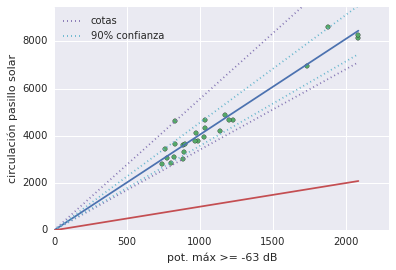
\includegraphics[width=0.5\textwidth]{Fig_fit_circulacion_por_jornada.png}
  \caption{
  sample size = 21, $p$ = 67
coef.corr.($s, c_p$) = 0.789206
$f$ = 0.339301, estimador de detección $f = 1/b$ asumiendo fitting $y = b x$
inf = 0.241768, sup = 0.414193, rango rel. = 0.508179
$f_5$ = 0.294769, $f_{95}$ = 0.373550, rango rel. = 0.232185
  }
  \label{fig:fitting_67}
\end{figure}

\item incrustar gráfico de $C$ vs $M$ todas las detecciones

\item incrustar gráfico de ajuste $C$ vs $M\big|^p$
\begin{figure}[H] 
  \centering
  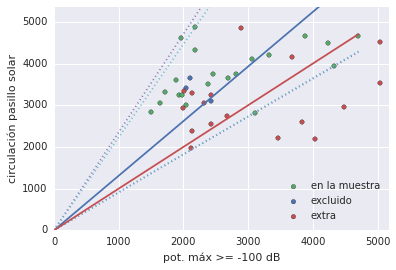
\includegraphics[width=0.5\textwidth]{scatter-sample-n-next.png}
  \caption{valores medidos después de la muestra en rojo
  }
  \label{fig:prediction}
\end{figure}

\end{itemize}

\[
f = \frac{M_A \Big|_{t\ge 0}^{p \ge -67dB}}{C}
\]

Aparentemente la distribución de circulación cambia para los nuevos días pero
las detecciones de los nodos se mantienen dentro de los rangos que estaban



Mediante el resultado de un estudio de 21 jornadas,
obtuvimos $\bar{f} = 0.35$ con confianza de $\beta = 0.90$,
eliminando los outlyers del 5to y 95vo percentil,
$0.31 \le \bar{f} \le 0.38$. Dando un error relativo 
\[
\frac{\bar{f}_{95}^p - \bar{f}_5^p}{\bar{p}} = 0.22
\]
(!) rever estos números


\begin{itemize}
\item incrustar gráfico de $M_c$ vs $p$ clusters detectados en función del la pot máxima
\item incrustar gráfico de $M_c$ vs $p$ clusters detectados en función del la pot máxima para los días individuales, de la muestra
\end{itemize}



\subsection{Visitas}
Nuestra difinición de visitas, se basa en personas q ingresan por más de 30 sec
por lo que usamos $t \ge 30$ segundos. Para calcular el umbral de potencia máxima $p$
usamos los datos anteriores como cota inferior o subestimador, 
ya que la problemática de un pasillo se asume que el factor de detección en el mismo 
es menor que al factor de detección de un local donde la gente permanece más tiempo en el.
\[
\bar{f} \le f^L_3 = f^L = \frac{M_L}{V} \le f^A
\]
Se puede tomar como cota superior el valor que se 
obtiene del valor mínimo observado 
$\widetilde{f^L} = \min_i M_i/C_i$ sin aplicarle ningún filtro
lo que nos da el supremo (la mínima cota superior)
durante los días de la muestra que es $0.60$ como se observa en la Figura~(\ref{fig:CotaSup})

\begin{figure}[H] 
  \centering
  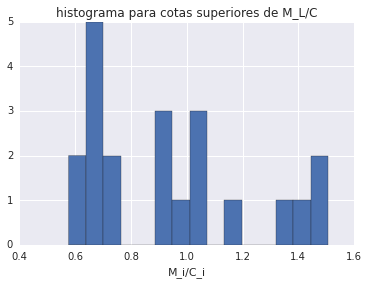
\includegraphics[width=0.5\textwidth]{cota_sup_hist.png}
  \caption{
    histograma de las posibles cotas superiores de $\frac{M_L}{V},
    \min_i \frac{M_i}{C_i} = 0.576125$
  }
  \label{fig:CotaSup}
\end{figure}

Vamos a tomar como factor de detección para la problemática del local $f$
como un promedio entre la cota inferior $\bar{f}$,
y la superior
\[
\bar{f}_{95} \le f_L \le \widetilde{f}
\] 
$F_L = (0.38 + 0.60)/2 = 0.44$.


\iffalse
Sin tener aún sufucientes mediciones \textit{in situ}, 
vamos a asumir que $\widetilde{f^L} = 0.5 \pm 0.25$
y considera un promedio ponderado de estas cotas $\bar{f} < \hat{f} <  \widetilde{f^L}$
y vamos a calcular un promedio ponderado 
$\hat{f} = \lambda \bar{f} + (1 - \lambda) \widetilde{f^L}$
entre 
los límites superior e inferior absolutos 
de los errores respectivos de las cotas:
$0.38 - 0.33 = 0.04$ y $0.5 - 0.25 = 0.25$
\[
\lambda = \frac{0.25}{0.28}\; (1 - \lambda) = \frac{0.03}{0.28}
\]
siendo 
\[
\hat{f} = \frac{0.25}{0.28} \bar{f} + \frac{0.25}{0.28} \widetilde{f^L} = 0.35
\]
(!) rever estos números


Para la
estimación de error del error se debe obtener más muestras \textit{in situ},
para que el intervalo de confianza de $\widetilde{f^L}$ no se superponga con el 
de $\bar{f}$
\fi

\begin{table}[]
\centering
\caption{My caption}
\label{my-label}
\begin{tabular}{lllllll}
 t  & p37 & p38 & sado & lu & ma & mi \\
 10 &  10 &  10 &    1 &  8 &  3 &  5\\
 11 &   5 &   5 &   25 &  7 &  6 &  3\\
 12 &   5 &   8 &    6 &  2 &  6 &  1\\
 13 &     &   3 &    8 &  3 &  4 & 11\\
 14 &   3 &   5 &   16 &  2 &  3 & 12\\
 15 &     &     &   26 & 11 & 10 &  7\\
 16 &  10 &  10 &   24 &  3 &  6 &  3\\
 17 &   3 &   3 &    8 &  8 &  9 &  7\\
 18 &     &   3 &   12 &  6 &  5 & 11\\
 19 &   8 &   8 &   10 &  5 & 16 & 10\\
 20 &   8 &  10 &   11 &  1 &  8 &  3\\
 21 &  15 &  20 &    1 &  2 &  4 &  4\\
 22 &     &     &    0 &  2 &  0 &  0\\
 total   & 67 &  85 &        74 & 60 & 80 & 77
\end{tabular}
\end{table}

\iffalse
----
Explicar las limitaciones q tenga el resultado

----
\fi
\paragraph{Algoritmo}
Para calcular o estimar las visitas $V$
escogimos el umbral $p$ para construir un filtro de detecciones
\[
\frac{M_L \Big|_{t\ge 30}^{p}}{V} \simeq \bar{f}
\]
observando los valores máximos, medios y mínimos de visitas en un muestreo.
\[
V = \bar{f} M \Big|^{t \ge 30}_{p \ge \hat{p}}
\]

(!) poner tabla de mediciones de empleados
\begin{figure}[H] 
  \centering
  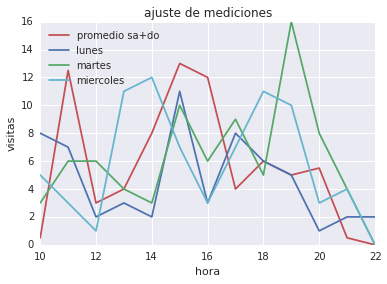
\includegraphics[width=0.5\textwidth]{mediciones.png}
  \caption{
    mediciones de visitas por hora tomados por empleados
  }
  \label{fig:mediciones}
\end{figure}


según los análisis de las Figuras~(\ref{fig:p_49-53})~y~(\ref{fig:p_51})
comparados con las mediciones tomadas \textit{in situ}
se decidió utilizar $\hat{p} = -51$dB.
\begin{figure}[H] 
  \centering
  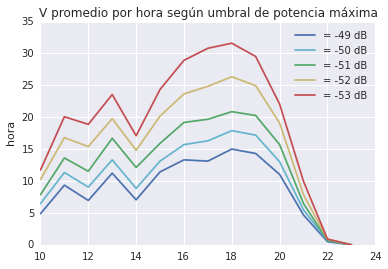
\includegraphics[width=0.5\textwidth]{p_49-53.png}
  \caption{
    promedio de mediciones por hora con distintos umbrales de potencias máximas dB.
  }
  \label{fig:p_49-53}
\end{figure}

(!) cambiar gráfico por los rangos de la potencia correspondiente


\begin{figure}[H] 
  \centering
  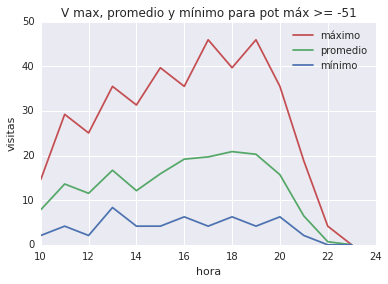
\includegraphics[width=0.5\textwidth]{p_51.png}
  \caption{
    máximo, promedio y mí­nimos de mediciones por hora con umbral potencia máxima $\ge -51$dB.
  }
  \label{fig:p_51}
\end{figure}

(!) cambiar gráfico por los de la potencia correspondiente


\iffalse
- visitas al local
Nuestra difimnicion de visitas (ejemplo: se basa en personas q ingresan por más de 30 sec) 
Estimación de error
Explicar las limitaciones q tenga el resultado
Explicar el algoritmo o familia de agoritmos. (Ejemplo: Estamos realizando el cálculo por hora o por día o ambos y como se relacionanó)
Prox pasos:

\fi


\subsection{ocupación y tiempo de permanencia}
Nuestra definición de ambas variables
sigue las mismas pautas que para la variable visitas (ejemplo: se basa en personas que ingresan por más de 30 sec) 

El cálculo de estas 3 variables tanto por jornada
como por hora,
se realiza a través de las visitas y funciones sql



\iffalse
Estimación de error
Explicar las limitaciones que tenga el resultado
Explicar el algoritmo o familia de agoritmos

- tiempo de permanencia
Nuestra definición de visitas (ejemplo: se basa en personas que ingresan por más de 30 sec) 
Estimación de error
Explicar las limitaciones q tenga el resultado
Explicar el algoritmo o familia de agoritmos

\fi

\subsection{Histogramas de potencias máximas}
\begin{figure}[H] 
  \centering
  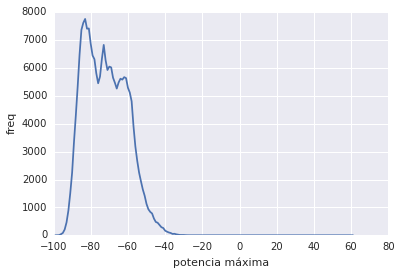
\includegraphics[width=0.5\textwidth]{pot_max.png}
  \caption{distribución de potencias máximas}
  \label{fig:pot_max_total}
\end{figure}

\begin{figure}[H] 
  \centering
  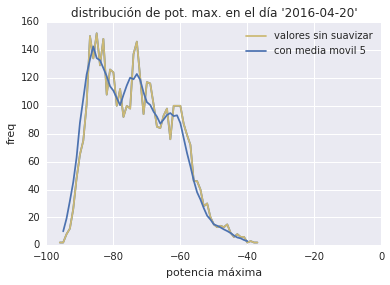
\includegraphics[width=0.5\textwidth]{pot_max_2016-04-20.png}
  \caption{distribución de potencias máximas de un solo día: el dia 20 de abril}
  \label{fig:pot_max_1_dia}
\end{figure}

\begin{figure}[H] 
  \centering
  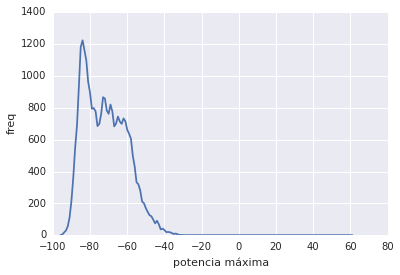
\includegraphics[width=0.5\textwidth]{pot_max_2016-04-10_al_16.png}
  \caption{distribución de potencias máximas de una semana: del 10 al 16/4}
  \label{fig:pot_max_semana}
\end{figure}

\begin{figure}[H] 
  \centering
  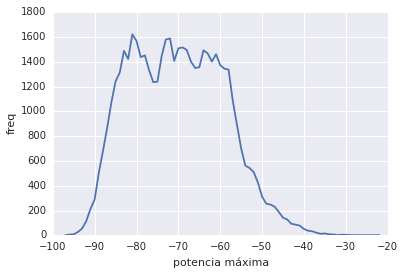
\includegraphics[width=0.5\textwidth]{pot_max_muestra.png}
  \caption{distribución de potencias máximas de la muestra}
  \label{fig:pot_max_muestra}
\end{figure}

\begin{figure}[H] 
  \centering
  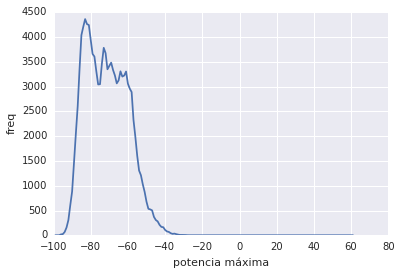
\includegraphics[width=0.5\textwidth]{pot_max_mes.png}
  \caption{distribución de potencias máximas de un mes: del 15/3 al 14/4}
  \label{fig:pot_max_mes}
\end{figure}




